% Instructions to change to html version:
% Comment out:
%  minipage, multicols,columnbreak, mathbf, hrule
% Replace all:% \begin{minipage}% %%\end{minipage} %%%%%\begin{mulicols}  %%%%%\end{mulicols}  %%%%\columnbreak % %%%%\begin{framed} %%%%%\endframed} %%%%%\hrule
% Search for \mathbf
% Replace \\] with \[ and \) with \(
% Enclose graphics in figure environments and add captions
% Re-tag \df environments as sections, subsections, etc.
% Command Line Code to Create html version:
%First: pdflatex -shell-escape filename.tex                                   
%Second, for each figure: inkscape "filename-figure1.pdf" -o "filename-figure1.png"
% Third: htlatex filename.tex "ht5mjlatex.cfg, charset=utf-8" " -cunihtf -utf8"


\documentclass[10pt]{article}

%\usepackage{tikz, pgf,pgfplots,wasysym,array}
%\usepackage{wasysym,array}

\usepackage{amsmath,amssymb}

\ifdefined\HCode
  \def\pgfsysdriver{pgfsys-tex4ht-updated.def}
\fi 
%\ifdefined\HCode
%  \def\pgfsysdriver{pgfsys-dvisvgm4ht.def}
%\fi 
\usepackage{tikz}
\usetikzlibrary{calc,decorations.markings,arrows}
\usepackage{pgfplots}

\pgfplotsset{compat=1.12}
\usepackage{myexternalize}
\usetikzlibrary{calc,decorations.markings,arrows}
\usepackage{framed}
\usepackage[none]{hyphenat}

\input{../../../common/1336_header_test.tex}

\begin{document}

\renewcommand{\myTitle}{MATH 2330: Multivariable Calculus}

\renewcommand{\mySubTitle}{4.4: Tangent Planes \& Linear Approximation }
%~\hfill Name: \underline{~~~~~~~~~~~~~~~~~~~~~~~~~~~~~~~~~~~~~~~~~~~~~~~}

\lectTitle{\vspace*{-.5in}\myTitle}{\vspace*{.1in}\mySubTitle \vspace*{-.25in}}




%\vspace*{-.5in}
\section*{Section 4.4 - Tangent Planes \& Linear Approximation, Part 1:}

%\hspace*{-.8in}\begin{minipage}{1.25\textwidth}
%\begin{framed}

\subsection*{Definitions \& Terminology:}
%\begin{multicols}{2}


\begin{figure}[htbp]
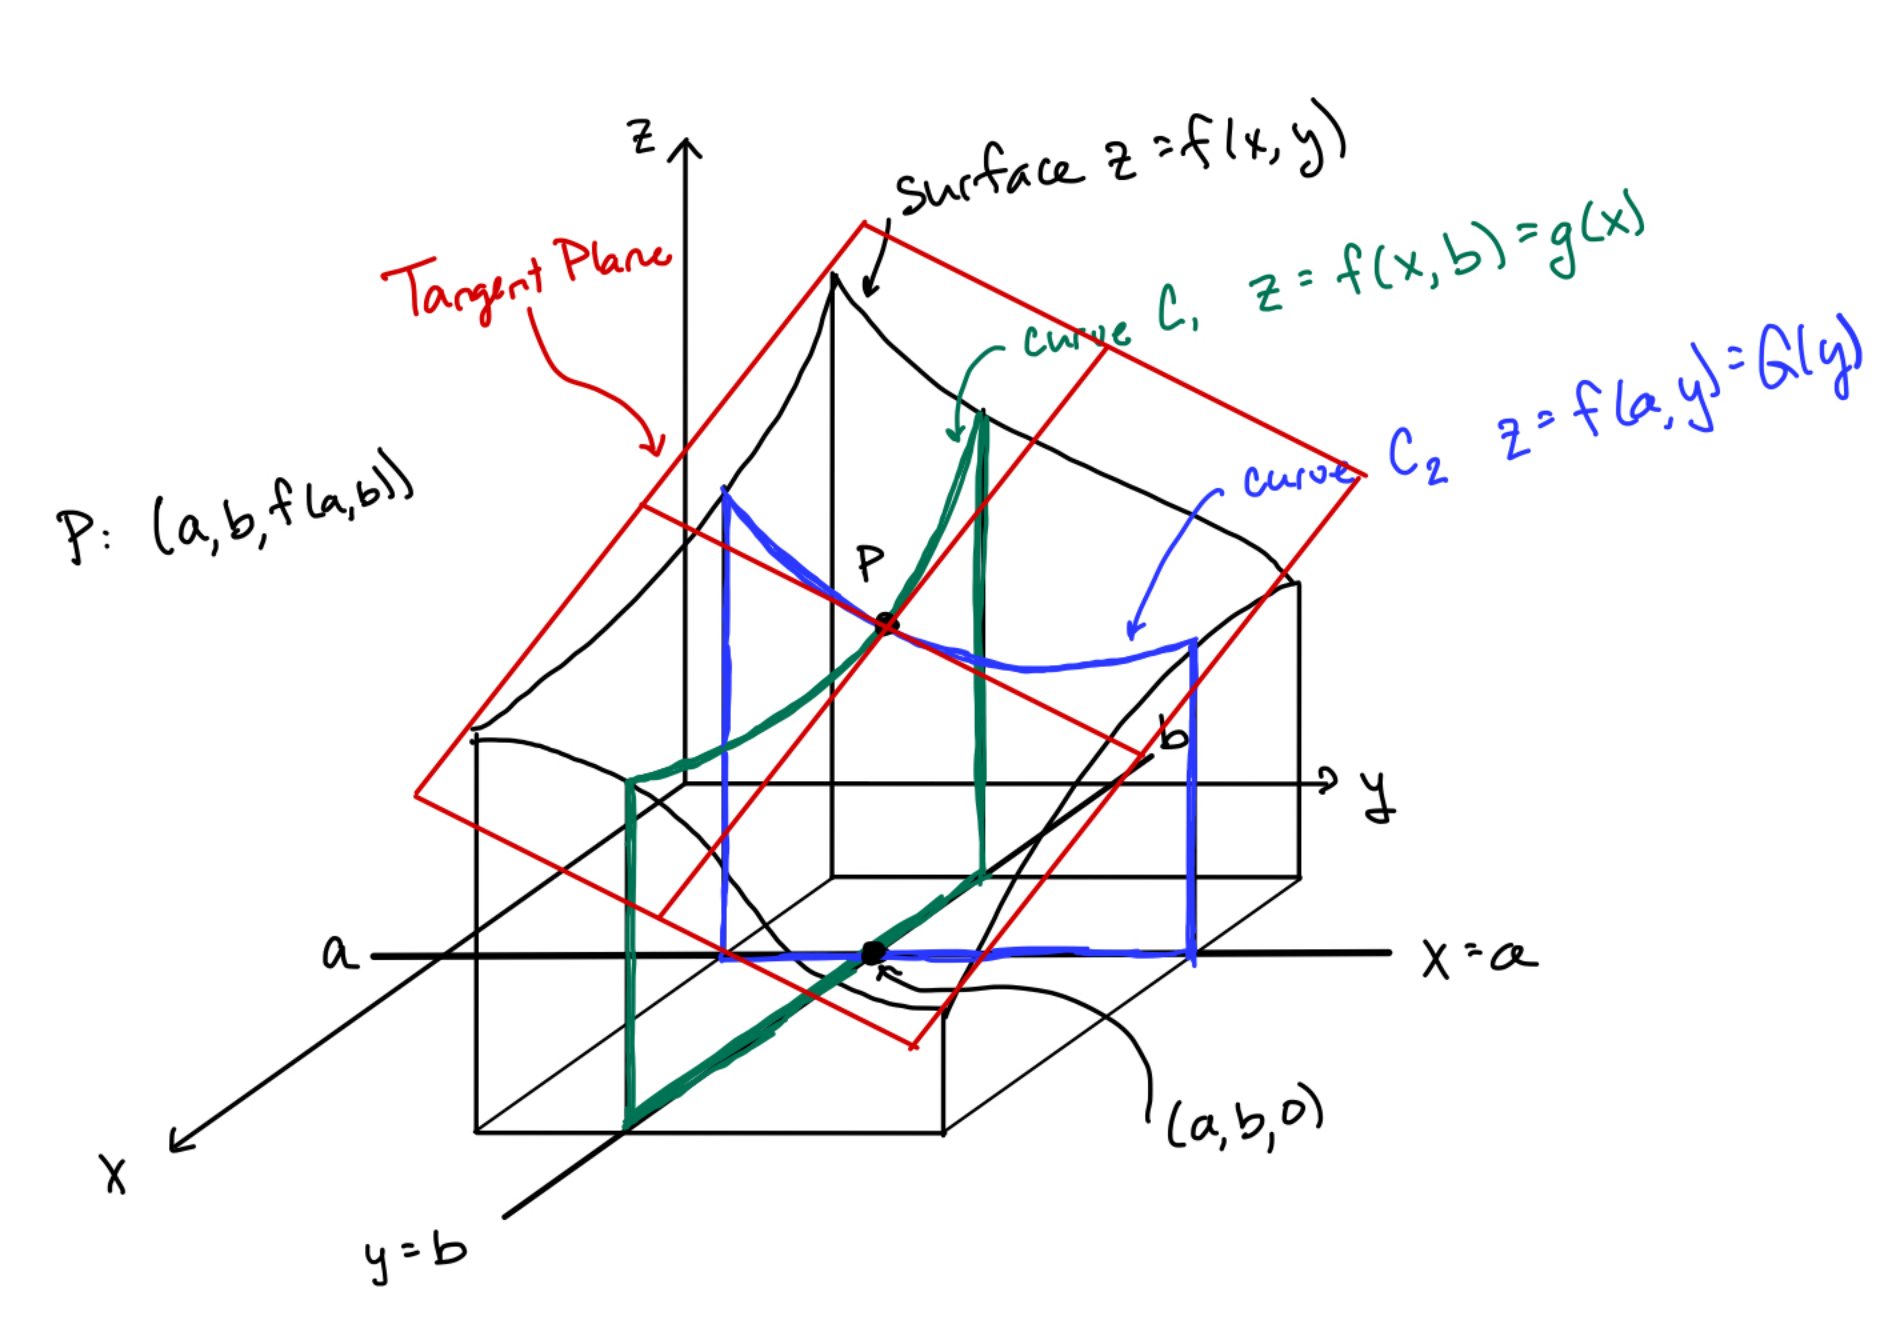
\includegraphics[width=.5\textwidth]{Tangent-Plane.png}
\caption{Tangent Plane Diagram}
\end{figure}


The \textbf{tangent plane} to the surface \(z=f(x,y)\) at the point \((a,b)\) is the plane defined by the tangent lines in the \(x-\) and \(y-\) directions at the point \((a,b)\).\\

The tangent plane gives the most accurate planar approximation to the surface at the point \((a,b)\).\\

\textbf{Tangent Plane Equation:}
\[z = f(a,b) + f_x(a,b)(x-a) + f_y(a,b)(y-b)\]

\textbf{Linearization of \(f\) at \((a,b)\):}
\[L(x,y) = f(a,b) + f_x(a,b)(x-a) + f_y(a,b)(y-b)\]

\textbf{Linear Approximation or Tangent Plane Approximation:}
\[f(x,y) \approx L(x,y) \]




%\end{multicols}


%\endframed}

%\end{minipage}




\begin{enumerate}[{Example} 1: ]
\item Consider the function \(f(x,y) = x^2y^3\).
\begin{enumerate}[(a)]
\item Find the equation of the tangent plane to \(z=f(x,y)\) at the point \((3,1,9)\).
\item Use Linear Approximation to estimate the value of \(f(x,y)\) at the point \((2.5,1.5)\).
\end{enumerate}

\end{enumerate}

\vfill \hfill \textit{(See Mathematica Demonstration!)}

\pagebreak



\section*{Section 4.4 - Tangent Planes \& Linear Approximation, Part 2:}

%\hspace*{-.8in}\begin{minipage}{1.25\textwidth}
%\begin{framed}

\subsection*{Definitions \& Terminology:}
%\begin{multicols}{2}

\begin{figure}[!h]

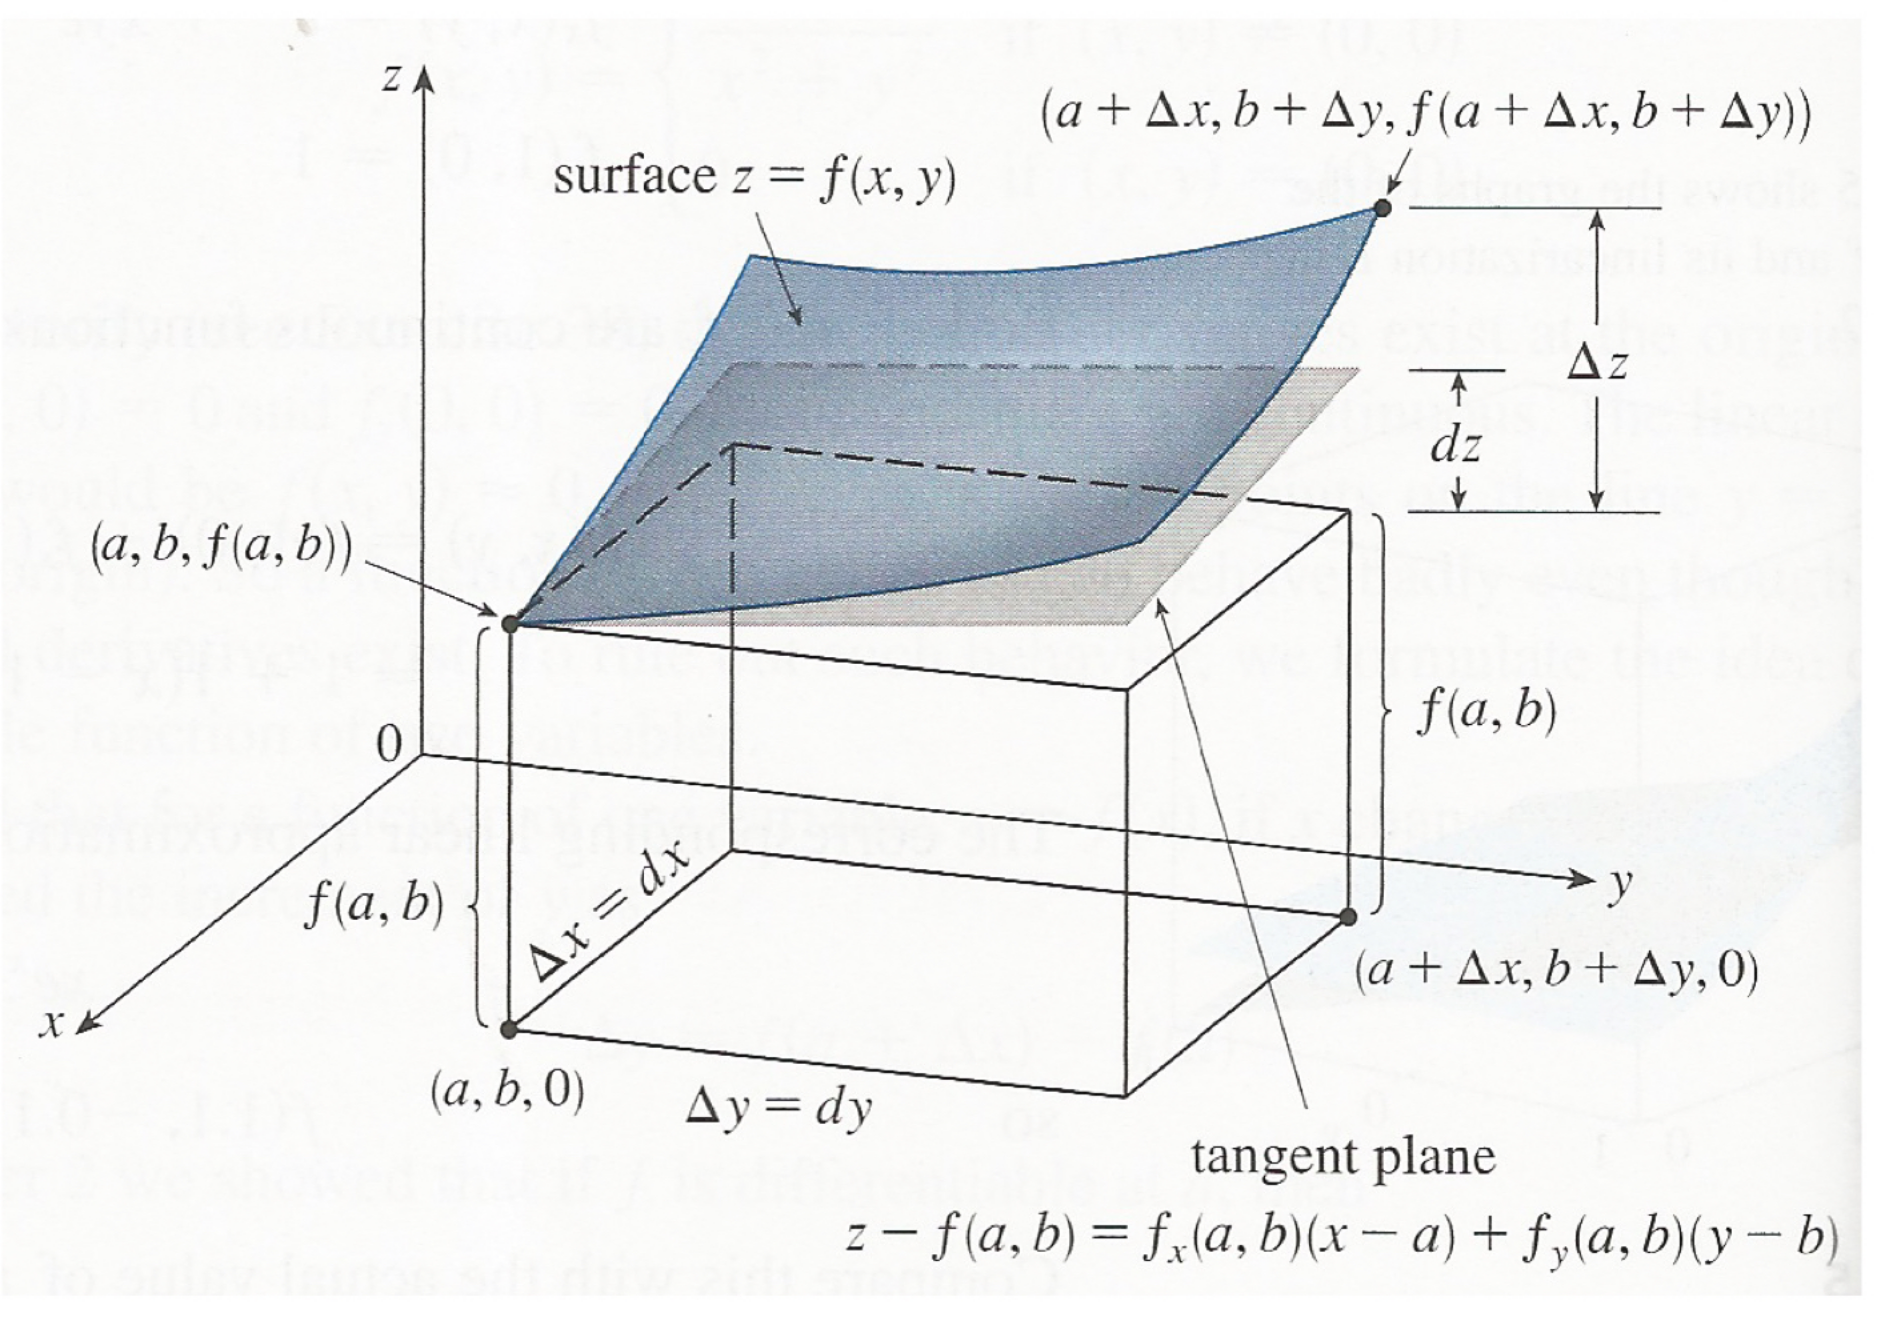
\includegraphics[width=.5\textwidth]{Tangent-Plane-Textbook.png}
\caption{Tangent Planes \& Differentials Diagram}
\end{figure}

\(\Delta z\): the change in height on the \textit{surface} \(z=f(x,y)\) that results from moving away from \((a,b)\) by \(\Delta x\) and \(\Delta y\).\\

\(dz\): the change in height on the \textit{tangent plane}, also called the \textbf{total differential}:
\[dz = f_x(a,b) dx + f_y(a,b) dy\]

\textbf{Differentiability:}

If \(z=f(x,y)\), then \(f\) is \textbf{differentiable} at \((a,b)\) if \(\Delta z\) can be expressed in the form
\[\Delta z = f_x(a,b) \Delta x + f_y(a,b)\Delta y + \varepsilon_1 \Delta x + \varepsilon_2 \Delta y\]
where \(\varepsilon_1\) and \(\varepsilon_2 \rightarrow 0\) as \((\Delta x, \Delta y)\rightarrow0\).\\

\textbf{Key Idea:} A function is differentiable at a given point if the tangent plane approximates the graph well near the point of tangency.

%\end{multicols}

%\hrule
\vspace*{.2in}

\subsubsection{Theorem: (Sufficient Condition for Differentiability)}
If the partial derivatives \(f_x\) and \(f_y\) exist near \((a,b)\) and are continuous at \((a,b)\), then \(f\) is differentiable at \((a,b)\).


%\endframed}

%\end{minipage}




\begin{enumerate}[{Example} 1: ]
\addtocounter{enumi}{1}
\item Give an example of a surface that is not differentiable at the origin.
\vfill

\item Find the total differential of \(f(x,y) = \cos(x^2 y)\)
\vfill

\end{enumerate}


\pagebreak

\section*{Group Work:}
\begin{figure}[!h]

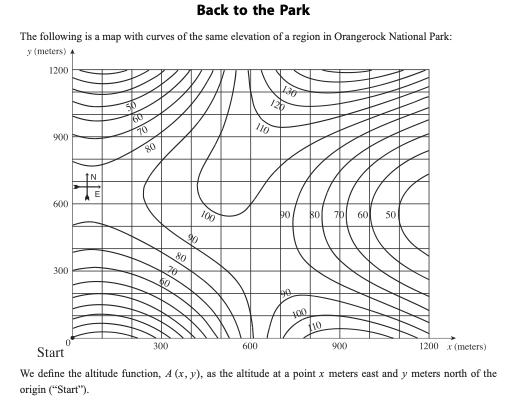
\includegraphics[]{Back-to-the-Park.png}
\caption{Contour Plot for "Back to the Park" Group Work Activity}
\end{figure}
\begin{enumerate}
\item Estimate \(A(300,300)\) and \(A(500,500)\).
\vfill
\item Estimate \(A_x(300,300)\) and \(A_y(300,300)\).
\vfill
\item What do \(A_x\) and \(A_y\) represent in physical terms?
\vfill

\item In which direction does the altitude increase most rapidly at the point \((300,300)\)?
\vfill

\item Use your estimates of \(A_x(300,300)\) and \(A_y(300,300)\) to approximate the altitude at \((320,310)\).
\vfill
\end{enumerate}


%\pagebreak
%
%\section*{Section 4.5: Chain Rule}
%
%%\begin{framed}
%\df{\textcolor{sblack}{Chain Rule, Case 1:}}
%Let \(z=f(x,y)\) where \(x=g(t), \quad y = h(t)\). Then\\
%\[\dfrac{dz}{dt} = \dfrac{\partial z}{\partial x} \dfrac{dx}{dt} + \dfrac{\partial z}{\partial y} \dfrac{dy}{dt} \hspace*{3in}\]
%%\endframed}
%
%\begin{enumerate}[{Example} 1: ]
%%\addtocounter{enumi}{1}
%\item (Revisited) Consider \(f(x,y)=x^2+y^2, \quad x=3t, \quad y = e^{2t}\). Compare the result from calculating \(\dfrac{df}{dt}\) using the Chain Rule with the result that you get from first rewriting \(f\) as a function of \(t\), then taking the derivative.
%\vfill
%
%
%\end{enumerate}
%
%%\begin{framed}
%\df{\textcolor{sblack}{Chain Rule, Case 2:}}
%Let \(z=f(x,y)\) where \(x=g(s,t), \quad y = h(s,t)\). Then\\
%\[\dfrac{\partial z}{\partial t} = \hspace*{4in}\] 
%
%\[\dfrac{\partial z}{\partial s} =\hspace*{4in}\]
%%\endframed}
%
%\begin{enumerate}[{Example} 1: ]
%\addtocounter{enumi}{1}
%\item Consider \(g(x,y)=x^2+xy+ y^2, \quad x=3(t+s), \quad y = e^{2st}\).
% Find \(\dfrac{\partial g}{\partial s}\) and \(\dfrac{\partial g}{\partial t}\) at \((s,t) = (1,0)\).
%\vfill
%
%\item Draw a diagram to help you write out the Chain Rule for\\ \(w=f(x,y,z)\) where \(x=g(s,t), \quad y = h(s,t), \qquad z=k(s,t)\).
%
%\vfill
%
%\end{enumerate}

\end{document}

